\documentclass{scrartcl}
\usepackage{fontspec}
\usepackage{polyglossia}
\setdefaultlanguage{german}
\begin{document}
\huge{Übungsblatt 00}
\newline
\newline
\newline
Aufgabe 1:
\newline
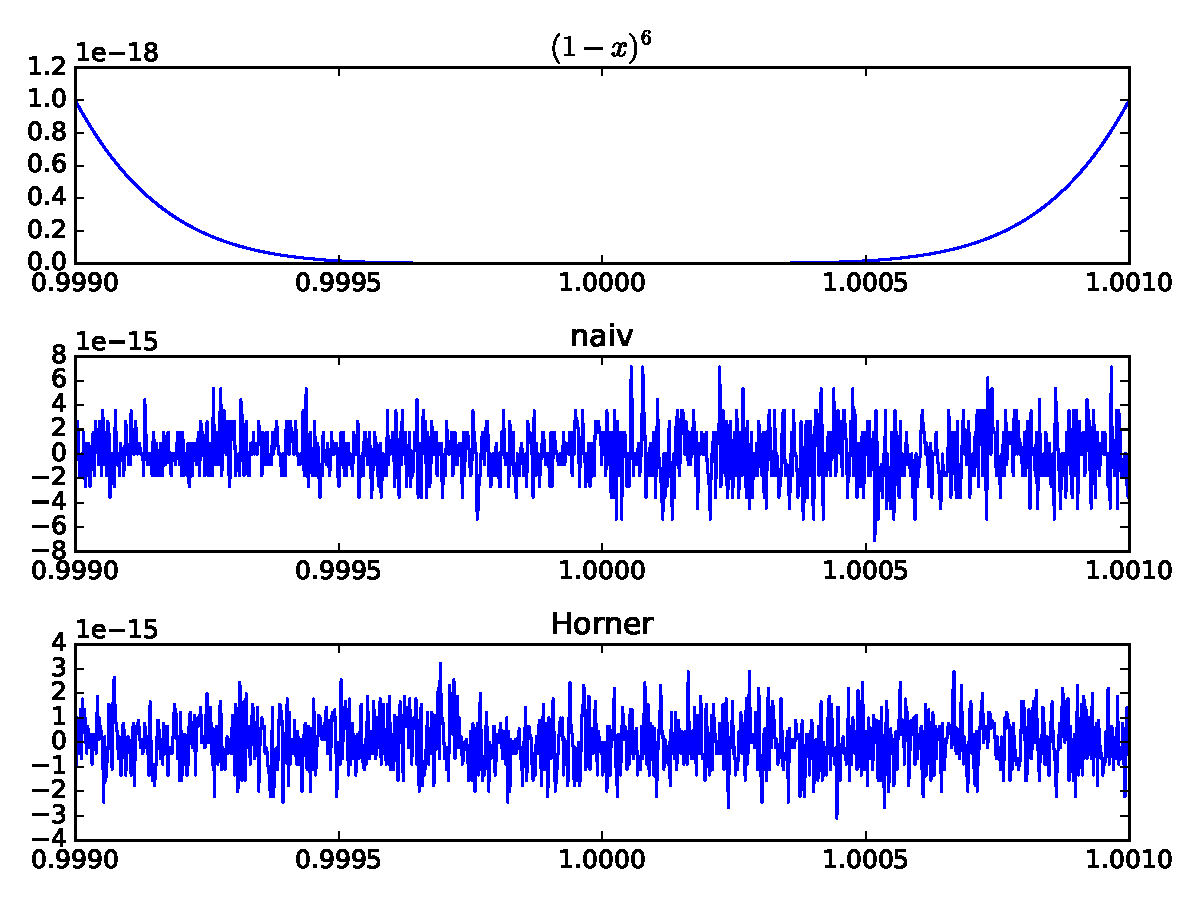
\includegraphics[width=0.7\paperwidth]{A1.pdf}
\newline
Interpretation:
\newpage
Aufgabe 2:
\newline
a)
\begin{equation}
lim_{x\rightarrow 0} (\sqrt{9-x}-3)/x = lim_{x\rightarrow 0} -1/(2\sqrt{9-x}) = -1/6
\end{equation}
\newline
b)\newline
$f( 0.1 ) = -0.167132219647\newline
f( 0.01 ) = -0.166712988701\newline
f( 0.001 ) = -0.166671296554\newline
f( 0.0001 ) = -0.166667129631\newline
f( 1e-05 ) = -0.166666712964\newline
f( 1e-06 ) = -0.166666671131\newline
f( 1e-07 ) = -0.166666667134\newline
f( 1e-08 ) = -0.166666680457\newline
f( 1e-09 ) = -0.166666680457\newline
f( 1e-10 ) = -0.166666680457\newline
f( 1e-11 ) = -0.166666680457\newline
f( 1e-12 ) = -0.166533453694\newline
f( 1e-13 ) = -0.164313007645\newline
f( 1e-14 ) = -0.17763568394\newline
f( 1e-15 ) = -0.44408920985\newline
f( 1e-16 ) = 0.0\newline
f( 1e-17 ) = 0.0\newline
f( 1e-18 ) = 0.0\newline
f( 1e-19 ) = 0.0\newline
f( 1e-20 ) = 0.0$\newline
Interpretation:
\newpage
Aufgabe 3:
\newline
a)
\newline Der numerische Wert für $f(x)$ weicht für $|x| > 40000$ um mehr als etwa $1\%$ vom algbraischen Wert ab.
\newline
b)
\newline Der numerische Wert für $g(x)$ weicht für $|x| < 0.00004$ um mehr als etwa $1\%$ vom algbraischen Wert ab.
\newline Der numerische Wert für $g(x)$ nimmt für $|x| < 0.00001$ den Wert 0 an.
\newline
c)
\newline
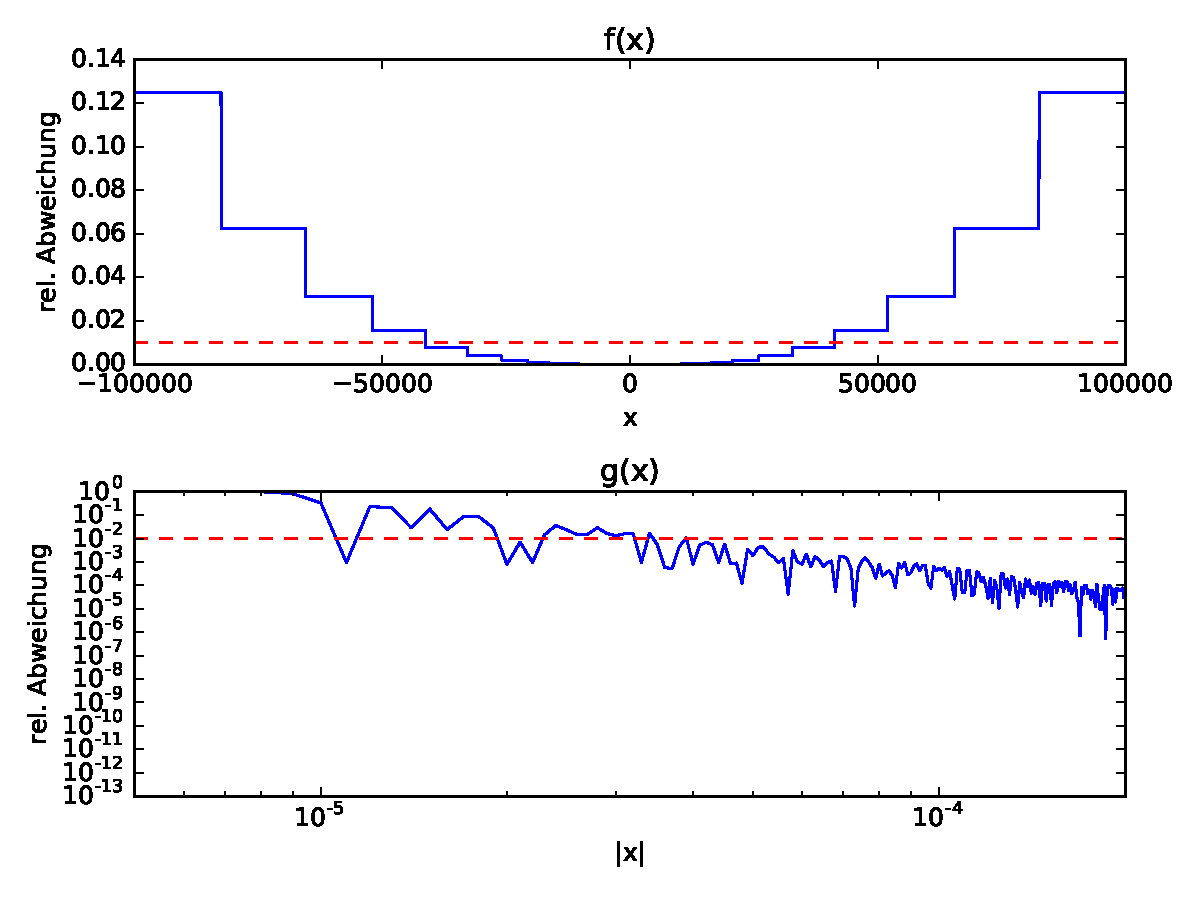
\includegraphics[width=0.7\paperwidth]{A3.pdf}
\newline
\end{document}